\subsection{%
  Теорема Уитни.%
}

\begin{theorem}
  \begin{align*}
    \vertexConnectivity{G} \le \edgeConnectivity{G} \le \minDegree{G}
  \end{align*}
\end{theorem}
\begin{proof}
  Сначала докажем левую часть этого неравенства. Рассмотрим минимальное по
  включению множество ребер \(E_{d}\), которые необходимо удалить для того,
  чтобы граф перестал быть связным.

  \begin{figure}[H]
  \centering
  
  \begin{subfigure}[b]{0.4\textwidth}

    \centering
    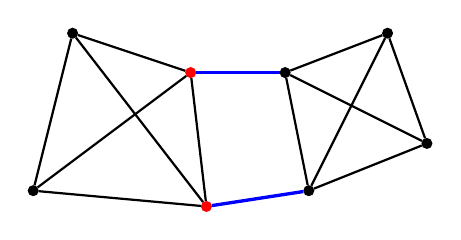
\begin{tikzpicture}[
  dot/.style = {
    shape = circle,
    fill = black,
    minimum size = 4pt,
    inner sep = 0pt,
    outer sep = 0pt,
  },
  every path/.style = {
    thick
  }
]
  \node[dot] (v1) at (-1, 0) {};
  \node[dot] (v2) at (-0.5, 2) {};
  \node[dot, fill = red] (v3) at (1, 1.5) {};
  \node[dot, fill = red] (v4) at (1.2, -0.2) {};

  \draw (v1) -- (v2) -- (v3) -- (v4) -- (v1) -- (v3);
  \draw (v2) -- (v4);

  \node[dot] (v5) at (2.5, 0) {};
  \node[dot] (v6) at (2.2, 1.5) {};
  \node[dot] (v7) at (3.5, 2) {};
  \node[dot] (v8) at (4, 0.6) {};

  \draw (v5) -- (v6) -- (v7) -- (v8) -- (v5) -- (v7);
  \draw (v6) -- (v8);
  
  \draw[very thick, color = blue] (v4) -- (v5);
  \draw[very thick, color = blue] (v3) -- (v6);
\end{tikzpicture}
    \caption{\(\vertexConnectivity{G} = \edgeConnectivity{G}\)}

  \end{subfigure}
  \qquad
  \begin{subfigure}[b]{0.4\textwidth}

    \centering
    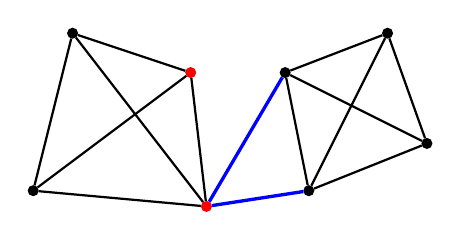
\begin{tikzpicture}[
  dot/.style = {
    shape = circle,
    fill = black,
    minimum size = 4pt,
    inner sep = 0pt,
    outer sep = 0pt,
  },
  every path/.style = {
    thick
  }
]
  \node[dot] (v1) at (-1, 0) {};
  \node[dot] (v2) at (-0.5, 2) {};
  \node[dot, fill = red] (v3) at (1, 1.5) {};
  \node[dot, fill = red] (v4) at (1.2, -0.2) {};

  \draw (v1) -- (v2) -- (v3) -- (v4) -- (v1) -- (v3);
  \draw (v2) -- (v4);

  \node[dot] (v5) at (2.5, 0) {};
  \node[dot] (v6) at (2.2, 1.5) {};
  \node[dot] (v7) at (3.5, 2) {};
  \node[dot] (v8) at (4, 0.6) {};

  \draw (v5) -- (v6) -- (v7) -- (v8) -- (v5) -- (v7);
  \draw (v6) -- (v8);
  
  \draw[very thick, color = blue] (v4) -- (v5);
  \draw[very thick, color = blue] (v4) -- (v6);
\end{tikzpicture}
    \caption{\(\vertexConnectivity{G} < \edgeConnectivity{G}\)}

  \end{subfigure}
\end{figure}

  В худшем случае придется удалить \(\abs{E_{d}} = \edgeConnectivity{G}\) вершин
  (по одной вершине на каждое ребро) чтобы граф перестал быть связным. Однако
  если существует вершины, при удалении которых удалится несколько ребер из
  \(E_{d}\), то можно будет удалить меньше вершин для достижения несвязности
  графа. Значит \(\vertexConnectivity{G} \le \edgeConnectivity{G}\).

  \begin{figure}[H]
  \centering
  
  \begin{subfigure}[b]{0.4\textwidth}

    \centering
    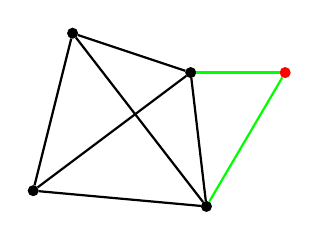
\begin{tikzpicture}[
  dot/.style = {
    shape = circle,
    fill = black,
    minimum size = 4pt,
    inner sep = 0pt,
    outer sep = 0pt,
  },
  every path/.style = {
    thick
  }
]
  \node[dot] (v1) at (-1, 0) {};
  \node[dot] (v2) at (-0.5, 2) {};
  \node[dot] (v3) at (1, 1.5) {};
  \node[dot] (v4) at (1.2, -0.2) {};

  \draw (v1) -- (v2) -- (v3) -- (v4) -- (v1) -- (v3);
  \draw (v2) -- (v4);

  \node[dot, fill = red] (v5) at (2.2, 1.5) {};
  \draw[very thick, green] (v5) edge (v3) edge (v4);
\end{tikzpicture}
    \caption{\(\edgeConnectivity{G} = \minDegree{G}\)}

  \end{subfigure}
  \qquad
  \begin{subfigure}[b]{0.4\textwidth}

    \centering
    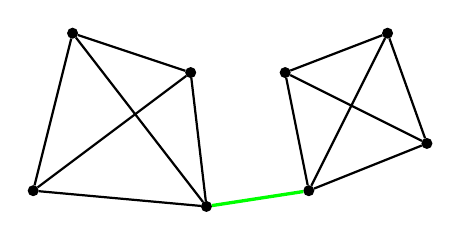
\begin{tikzpicture}[
  dot/.style = {
    shape = circle,
    fill = black,
    minimum size = 4pt,
    inner sep = 0pt,
    outer sep = 0pt,
  },
  every path/.style = {
    thick
  }
]
  \node[dot] (v1) at (-1, 0) {};
  \node[dot] (v2) at (-0.5, 2) {};
  \node[dot] (v3) at (1, 1.5) {};
  \node[dot] (v4) at (1.2, -0.2) {};

  \draw (v1) -- (v2) -- (v3) -- (v4) -- (v1) -- (v3);
  \draw (v2) -- (v4);

  \node[dot] (v5) at (2.5, 0) {};
  \node[dot] (v6) at (2.2, 1.5) {};
  \node[dot] (v7) at (3.5, 2) {};
  \node[dot] (v8) at (4, 0.6) {};

  \draw (v5) -- (v6) -- (v7) -- (v8) -- (v5) -- (v7);
  \draw (v6) -- (v8);
  
  \draw[very thick, color = green] (v4) -- (v5);
\end{tikzpicture}
    \caption{\(\edgeConnectivity{G} < \minDegree{G}\)}

  \end{subfigure}
\end{figure}

  Далее докажем правую часть этого неравенства. В худшем случае, чтобы получить
  несвязный граф, потребуется удалить все ребра инцидентные вершине с наименьшей
  степенью. В этом случае \(\edgeConnectivity{G} = \minDegree{G}\). Однако
  бывают графы, в которых \(\edgeConnectivity{G} < \minDegree{G}\).
\end{proof}
